\documentclass[12pt,a4paper]{report}

% ==== PACKAGES ====
\usepackage{graphicx}
\usepackage[parfill]{parskip}
\usepackage{hyperref}
\usepackage{upquote}
\usepackage[font=small,labelfont=bf]{caption}


%======= LISTINGS =========
\usepackage{listings}
\usepackage{color}

\definecolor{dkgreen}{rgb}{0,0.6,0}
\definecolor{gray}{rgb}{0.5,0.5,0.5}
\definecolor{mauve}{rgb}{0.58,0,0.82}

\lstset{frame=tb,
  language=Java,
  aboveskip=3mm,
  belowskip=3mm,
  showstringspaces=false,
  columns=flexible,
  basicstyle={\small\ttfamily},
  numbers=none,
  numberstyle=\tiny\color{gray},
  keywordstyle=\color{blue},
  commentstyle=\color{dkgreen},
  stringstyle=\color{mauve},
  breaklines=true,
  breakatwhitespace=true,
  tabsize=3
}

%===== MACROS ====
\newcommand{\code}[1]{\fbox{\texttt{#1}}}
\renewcommand{\baselinestretch}{1.3} 

%====== SETTINGS =====
%\renewcommand{\familydefault}{\sfdefault}


% ===== TITILE PAGE ====
\title{TypeScript - front to back}
\author{Daniel Niederberger}
\begin{document}
\begin{titlepage}
	\centering
	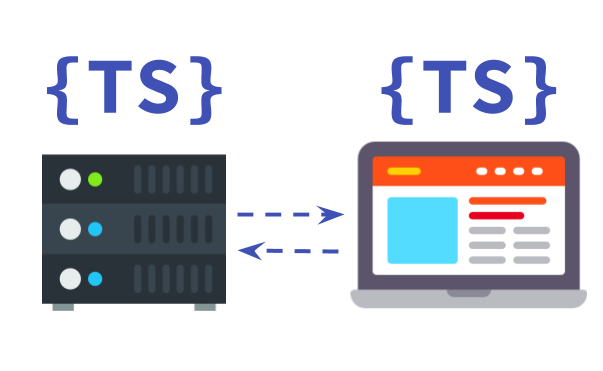
\includegraphics[width=1\textwidth]{figures/cover-image.png}\par
	% {\scshape\LARGE A TSMEAN Book \par}
	%\vspace{1cm}
	%{\scshape\Large Version 1\par}
	\vspace{1.5cm}
	{\huge\bfseries TypeScript \\ \Huge{Front to Back}\par}
	\vspace{2cm}
	{\Large\itshape Daniel Niederberger\par}
	%\vfill
	%reviewed by\par
	%Dr.~Franz \textsc{Ösinger}

	\vfill

% Bottom of the page
	{\large \today\par}
\end{titlepage}

\tableofcontents
\newpage

\chapter*{Prologue}
Welcome to the emerging world of full stack TypeScript! You are probably familiar with TypeScript from the frontend, usually in conjunction with Angular. While Angular played a large role in making the TypeScript language more popular, TypeScript is not limited to the Frontend. Nowadays there are runtime environments for JavaScript (and TypeScript compiles to JavaScript) so you can also write TypeScript for the backend. This book is about having TypeScript on both sides, frontend and backend. It's about how to build a medium- to large-sized web-application with full stack TypeScript the right way.

Who's this book for? The first chapter is crucial for decision makers. If you're the person in charge of deciding what stack you're going to use to build the next app of your team, it's important to understand the strengths and weaknesses of the stack. A stack will accompany you down the road, so careful consideration is necessary. Is full stack TypeScript the right choice for you? The first chapter tries to answer that question.

Once the decision to go with full stack TypeScript is made, developers need to learn how to set up their projects and work with full stack TypeScript. The rest of the book is about gaining a deeper understanding of the inner works of full stack TypeScript for developers. A special focus is put on the backend, since ``TypeScript in the backend'' is what people usually are least familiar with.

\chapter{Is Full Stack TypeScript Right for You?}

When it comes to web application, after you have decided what you want to build, the next decision is \textit{how} to build it. That's the decision of the tech stack you're going to use. It's a decision that shouldn't be taken lightly, as it will have a strong lock-in effect no matter how modular you're going to build your code. As your codebase grows, it becomes more and more work to migrate away to another technology. For smaller projects that might not be too much of a problem, since a complete or partial rewrite can be done fairly quickly, but for larger codebases the cost of migration becomes gruesome. So as a decision maker, you should be well informed of the strengths and weaknesses of your choice.

Now from my experience, one of the most important factors to consider is your team. If you have people with years in one technology that are happy with that technology, then my first recommendation would be to back away. This doesn't just hold true for TypeScript, it also holds true for example to forcing Python developers to program in Java. One of the most important factors to making full stack TypeScript work in your team is, that they \textit{must be open to experimentation}. They must like the idea of working full stack TypeScript in principle. If you're forcing them to do it, you'll have an uphill battle. The team must be willing to learn new things, try out things, make mistakes and live with large uncertainty in a rapidly changing environment. They shouldn't have inflated expectations of what the change will bring them, so they're not discouraged when first problems arise, since they knew what they were getting into. Every choice comes with ups and downs, and so does going full stack TypeScript. Just make sure everybody fully agrees to going down this road. To help you and your team make this decision, I'm analysing strengths, weaknesses, opportunities and risks of going full stack TypeScript here.

\subsection{The Weaknesses and Risks}

When going full stack TypeScript you should be aware that \textit{not many people have done this before}. You will be a pioneer. There are \textit{some} large projects written in TypeScript though. The largest one I'm aware of is Microsoft's IDE ``VS Code'' with around 350'000 lines of TypeScript code. Then there's Angular\footnote{Throughout this book ``Angular'' refers to the newer framework, i.e. Angular2, Angular4 and so on. The old framework is referred to as ``AngularJS''.}, the frontend framework by Google clocking in around 250'000 lines of TypeScript code, but this again is only for the frontend and not full stack. Another large project is Babylon.js with around 200'000 lines of TypeScript code. As you can see, there are ``large'' TypeScript projects, but then again, not that many. It dwarfs in comparison to the billions of lines of Java, Python, PHP and JavaScript code that have been written. Then again, just because there exists a lot of JavaScript code doesn't mean it's better than TypeScript, it's just been around for longer. I would argue that the world is a changing place and you'll never be sure what's the next big thing. The roman empire was great once, but it's not anymore. AngularJS was great once, it's not anymore. You just can't be sure.

However, this doesn't help with that fact that pioneers have a hard life. Even though the US is a powerful country now, when Columbus first arrived he for sure had a harder time than when he'd just stayed in Spain. It's the same with full stack TypeScript. You're on \textit{new land}, in a place where few people have set foot before. This means there aren't really best practices or they might change over time. No-one knows what they're doing, really. You'll make mistakes since you can't learn from others. There's not too much documentation to guide you through the process (this book being the exception, of course). While the documentation on full stack TypeScript is almost non-existent at this point, the documentation on TypeScript in general is surprisingly good for a language this young. There's the official TypeScript docs which is quite good, there are several online tutorials and there are a couple of online courses as well.

The whole TypeScript ecosystem is young and unstable. Packages are being broken and deprecated frequently and often they are buggy. The whole ecosystem is quite open source oriented and people will often work on it in their spare time. There's a lot of passion in the projects, but at the same time the lack of resources and professionalism is notable. A battle tested ORM (object-relational mapping) tool like Hibernate for Java doesn't exist.\footnote{There's typeorm (\url{https://github.com/typeorm/typeorm}) but it's still younger than an unhatched chicken.} There's no backend framework like Java's Spring or Python's Django.\footnote{There's NEST (\url{https://github.com/nestjs/nest}) but it's a one-man show so far.}

To top it all off, TypeScript isn't made to be highly performant. TypeScript is compiled, but unlike other languages it doesn't compile to bytecode, instead it compiles to \textit{JavaScript}. Then JavaScript, a dynamic language, is executed by Node.js, the browser or another JavaScript runtime environment. Now while there are quite good JavaScript engines out there, it's hard for them to match the performance of languages that are compiled to bytecode, like Java or Rust.

Writing concurrent code \textit{might} be considered as weakness or weaknesses of full stack TypeScript. That is because this would traditionally be handled with callbacks, which are a surefire way to callback hell. However, the recent addition of the \texttt{async / await} syntax to the JavaScript language alleviates some of the pain in terms of readability and maintainability. Like this, TypeScript + Node.js is an easier road to concurrency than, let's say, with Java because all packages available are already written non-blocking. On the other hand, languages like Go or Scala have concurrency baked into them with more sophisticated models than callbacks. 

Wow, that were a lot of points discouraging from full stack TypeScript so far, enough for anyone risk averse to decline doing a project in full stack TypeScript. However, there are also a lot things going in favor of full stack TypeScript!

\subsection{The Strengths and Opportunities}
People are switching from JavaScript to TypeScript in many places. Angular switched to TypeScript, so did RxJS, so did ui-router and so on. This is a good sign, it's an indicator that using TypeScript could be really beneficial to projects as opposed to JavaScript. So when you were considering doing your project full stack JavaScript with a node.js backend, then people switching the language in the frontend should make you think why not also switch it in the backend? TypeScript has many advantages over JavaScript, the most important one for me being that it better documents your program for yourself and your team. Types shine at communicating intent, which becomes especially important for pieces of code that should be long lived and viewed by many eyes.

But what if you weren't planning on doing a JavaScript backend, what if the competition is a Java, Python or PHP backend? Why on earth would you sacrifice such battle tested backend languages for something with all the downsides previously discussed? To me the major point is this one: one language everywhere. One language everywhere comes with an incredible host of benefits. Your developers only need to know one language. Your frontend and backend devs can communicate better. You don't even need the separation frontend / backend devs anymore, you can also operate in ``problem solving teams''. On small-sized projects, a single developer can maintain the project without ever needing to switch context when doing backend / frontend work. A single developer can develop a feature back to front. You can have one style guide for the entire project. You can have one package management solution for the entire project. You can have code shared between the backend and frontend, such as utility functions or interfaces. You can easily migrate routines from the backend to the frontend or vice versa.

Now the ``one language everywhere'' possibility isn't exactly new, it's been around for a couple of years with JavaScript and node.js or also GWT. With JavaScript and node.js, the counter argument often was ``Why sacrifice a good language like Java or Python for something terrible like JavaScript?''. But first of all, the JavaScript language has evolved since then, and second, with TypeScript you'll get an additional boost in useful features. So if you actually think the TypeScript programming language holds water to Java or Python or any other backend language, like I do, then there isn't standing much in the way (except for the points with the documentation and adoption and so on...).

Another benefit, depending on how you look at it, is that with a backend in TypeScript + Node.js, you can handle concurrency. You could have thousands of clients connected to your server with little resources since Node.js is single threaded and non-blocking, which is for example a requirement for a real time chat app. With a threaded backend, your servers would run out of memory pretty quickly. It's not impossible to do this in other languages, I'm just saying it's baked right into Node.js.

Now we can see that full stack TypeScript offers a lot of benefits, but why should you go for it now, when no one else has tried and tested it? It's true that it's a risky bet. But if it should prove useful to you, and you can really benefit from ``one language everywhere'' and over time more people adopt this and the ecosystem will get better, in a few years you'll be in a strong position.

\subsection{Conclusion}
I hope I could shed some light on what it entails to going full stack TypeScript. You could see that there are a lot of different aspects that have to be considered. Now, the decision is up to you. If the ``one language everywhere'' benefits outweigh the ``being-a-pioneer'' problems and risks and your team is up for it, then go for it. Otherwise, you can also build your next web application with the technologies you're used to and see how the environment evolves over the next couple of years and reevaluate then. What I wouldn't recommend is basing your choice strongly on performance considerations. It is very hard to estimate your use cases correctly beforehand such that you could see whether you'd get a performance gain or loss using a backend written in TypeScript. There is always the possibility of rewriting parts of the application causing bottlenecks in another language, which you may then choose in a way to be perfect for that job.

\chapter{Fundamentals}
\label{chapter:fundamentals}

In case you had enough exposure with TypeScript to feel safe with the fundamentals of it, feel free to skip this chapter. Otherwise, here are the fundamentals of TypeScript put together in a short tutorial, such that you can learn the fundamentals of TypeScript quickly. This tutorial aims at covering the most relevant parts, rather than at being exhaustive.

\section{What is TypeScript?}

TypeScript is a \textbf{programming language} that compiles to JavaScript. So in order to run a program that is written in TypeScript, it is first compiled into JavaScript and the JavaScript code is executed either by a browser or by a server-side JavaScript runtime like Node.js.

Now TypeScript isn't the first language that is compiles to JavaScript, another popular example of a language that compiles to JavaScript is CoffeeScript. So this begs the question, what's different about TypeScript? First of all, TypeScript is a \textbf{superset} of JavaScript.
\begin{figure}
\centering
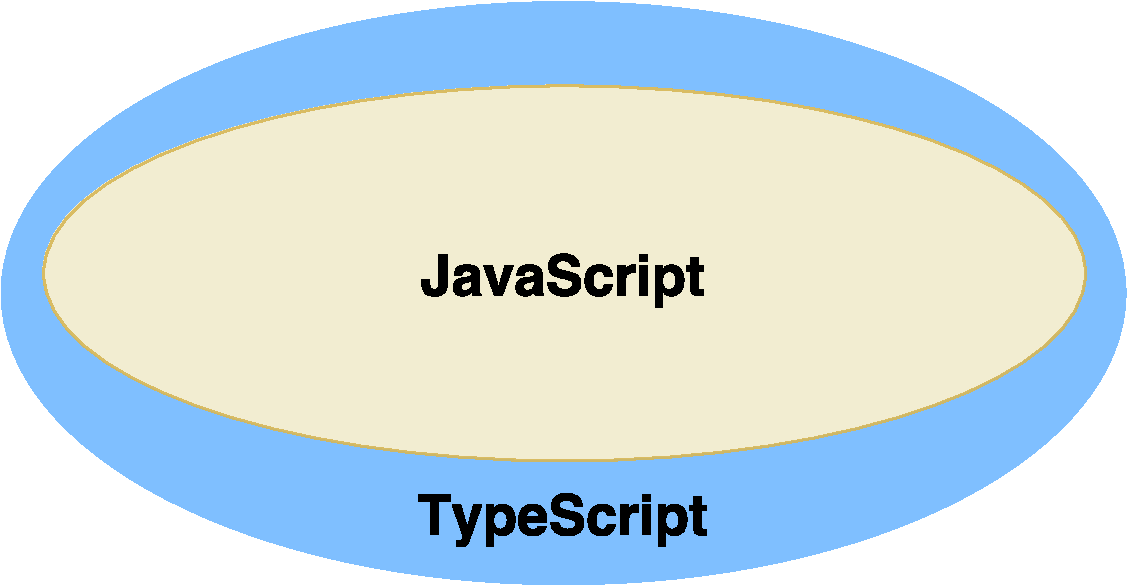
\includegraphics[scale=0.5]{figures/ts-js-diagram.pdf}
\caption{TypeScript is a superset of JavaScript.}
\end{figure}
That means that valid JavaScript is valid TypeScript, so everything that TypeScript offers are \textbf{additions} to the JavaScript language. Now the previous statement was a bit simplified for didactical purposes. You may run into compilation errors when trying to compile regular JavaScript with the TypeScript compiler. But unlike other compilers that won't produce an output when there are errors, the TypeScript compiler still produces a JavaScript output. That means the completely correct statement would be ``Valid JavaScript can be compiled by the TypeScript compiler to JavaScript''. This sounds quite stupid, but it has some nice implications. For one, you can start using TypeScript by renaming your JavaScript files (if you have any) from \texttt{myfile.js} to \texttt{myfile.ts}. Second, this isn't the case for every language that can be compiled to JavaScript. For example if you will have JavaScript in your CoffeeScript code, it usually won't compile at all. All of that means that the entry barriers to TypeScript are kept to a minimum. You don't have to learn a new language if you already know JavaScript, you just have to learn the additions that TypeScript brings to the language. What those additions are  is covered later in this chapter.

There's a second purpose to TypeScript than enhancing JavaScript with additional options. JavaScript is a language that strongly evolved over the years, but older browsers only understand old versions of JavaScript. To solve this problem we need something that is able to compile newer versions of JavaScript to older versions of JavaScript. TypeScript is capable of doing this. When setting up TypeScript you can specify to \textit{which version of JavaScript} it should compile. So you could write write TypeScript on the basis of ES7 (the newest version of JavaScript) and compile it to ES5, a version that's compatible with most browsers. Actually it is a little more complicated than that, because there are some constructs that can't be translated and need to be polyfilled (see XXX), but for the majority of concepts TypeScript can translate ES7 or ES6 to older versions of JavaScript.

So to summarize, TypeScript does two things for you:
\begin{enumerate}
\item{It extends JavaScript with new features, most notably types}
\item{It can compile ES7 / ES6 to ES5 such that you can benefit from the features of the newer JavaScript versions while still staying compatible with older browsers.}
\end{enumerate}

In the following we're going to explore the new features that TypeScript brings us. When you're coming from a ``plain old JavaScript'' background and have neither experience with ES6 / ES7 nor with TypeScript, it's often confusing where a concept comes from. Is it from ES6 / ES7 and merely made accessible to you by TypeScript (you know, the translating ES6 to ES5 story) or is it actually \textit{only} available in TypeScript? This tutorial tries to distinguish clearly between the two.


\section{Types}

So now we know that TypeScript compiles to JavaScript and that it's furthermore a superset of JavaScript that offers some additions. So what are those additions then? As the name ``TypeScript'' suggests, one of the most important additions are \textbf{types}. For optionally typed languages such as TypeScript, types are often referred to as ``type annotations''.

JavaScript has no types, so if you assign, for example, a number in JavaScript you'd just write \code{var x = 5}. In TypeScript however, you can assign a type to this variable, so you would write \code{let x: number = 5}. Here, \code{number} declares the type of the variable. We have also replaced \code{var} with \code{let} since that's the new industry standard to define variables for ES6 or above.\footnote{The \code{var} keyword has function scope whereas the \code{let} keyword is block scoped. Those concepts have nothing to do with TypeScript, but rather with different versions of JavaScript. The keyword \code{let} was introduced in ES6 while \code{var} has been there since the beginning.} There are predefined types that can be extended with your own types, classes and interfaces.

\subsection{Booleans, Numbers and Strings}
The most basic predefined types are \texttt{boolean}, \texttt{number} and \texttt{string}. Here are some examples:
\begin{lstlisting}
let isCute: bool = true;
let numberOfBunnies: number = 25;
let nameOfFavoriteBunny: string = 'Lindy';
\end{lstlisting}

\subsection{Arrays}
The next most important type is the array. Arrays are denoted by appending square brackets:
\begin{lstlisting}
let bunnies: string[] = ['Lindy', 'Jacker', 'Nobler', 'Frenzy'];
\end{lstlisting}

\subsection{Any}
TypeScript offers you a way to declare variables that may change their type. That way you can still employ ``duck typing'' where you want to.
\begin{lstlisting}
let justAboutAnything: any;
justAboutAnything = 5; // OK
justAboutAnything = 'hello' // OK
justAboutAnything = () => {console.log('hello')} // OK ...
\end{lstlisting}
It would also work to just leave away the \code{any}-keyword here, but with it present it's more explicit that this variable is actually expected to change it's type on runtime. There is a TypeScript compiler option \code{noImplicitAny} which makes it illegal to not explicitly declare where types are expected to be dynamic with the \code{any} keyword.


\subsection{Functions}
Functions are at the heart of JavaScript since the beginning. To just declare the input and output types function, the following syntax is used:
\begin{lstlisting}
// declaration of a function
let additionFunction: (x: number, y: number) => number;
\end{lstlisting}
As usual, the start of the type annotation is denoted by the colon. Next follows a pair of round parenthesis that include the names of the arguments and their respective types. In the example above, we have a function that takes two arguments named \texttt{x} and \texttt{y}, both being of type \texttt{number}. The next element in this function declaration is the \textbf{fat arrow} \code{=>}, followed by the return type of the function, in the example the return value is also expected to be of type \texttt{number}.

Declaring functions is especially useful when defining interfaces, see XXX. What is also used often is assigning an anonymous function to a variable.

Adding types to an anonymous function is as easy as adding the types to all arguments:
\begin{lstlisting}
(x: number, y: number) => {
  return x + y;
}
\end{lstlisting}
Note that we're using the ES6 fat arrow syntax here instead of the traditional \texttt{function}-keyword.

A very common coding style is to assign anonymous functions to variables. In this case, we would have:
\begin{lstlisting}
let additionFunction = (x: number, y: number) => {
  return x + y;
}
\end{lstlisting}

The attentive reader might have noticed, that here we define one type less than in the type declaration above: the return type of the function is never specified explicitly. This is pretty ok though, since TypeScript is using \textbf{type inference} so it still knows that the output of this function will be of type number.

\begin{figure}
\centering
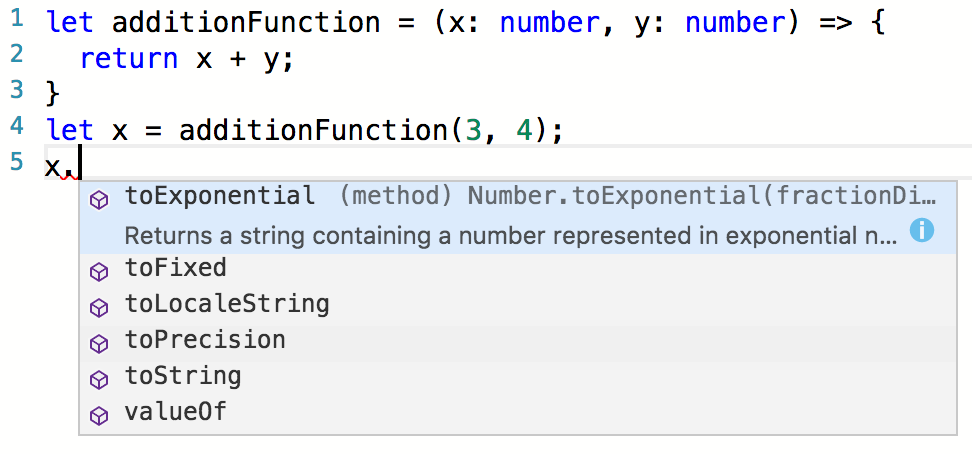
\includegraphics[scale=0.7]{figures/typeinference.png}
\caption{Screenshot from the TypeScript Playground. Through type inference TypeScript knows that the output value of the \texttt{additionFunction} will have type \texttt{number}.}
\end{figure}

In case you prefer to be explicit, you can still add a type declaration to the variable declaration as shown at the beginning of this section, but the code will get more lengthy.

\subsubsection{Optional Arguments}
By default all arguments in a TypeScript function are required. For example, if you tried to leave away one of the inputs of the above \texttt{additionFunction}, the compiler would throw an error.
\begin{lstlisting}
let additionFunction = (x: number, y: number) => {
  return x + y;
}
additionFunction(3); // ERROR: Expected 2 arguments, but got 1.
\end{lstlisting}
To make arguments optional, you can use a question mark \code{?} after the name of the argument:
\begin{lstlisting}
let sayHello = (name?: string) => {
  name ? console.log(`Hello ${name}!`) : console.log('Hi there!')
}
sayHello(); // 'Hi there!'
sayHello('Peter') // 'Hello Peter!'
\end{lstlisting}

\subsection{Objects}
Another age old construct in JavaScript are Objects. Objects are simply put just key-value pairs. Just so we're on the same page, we're talking about this construct:
\begin{lstlisting}
let car = {
  color: 'green',
  startEngine: () => {
    // ... do some stuff
  }
}
\end{lstlisting}

So how can you provide type annotations for objects? Since you usually know exactly how your object is going to look like, you'd typically do this with an interface or a class, which we're covering in more detail in XXX.
\begin{lstlisting}
let car: Car = {
  color: 'green',
  startEngine: () => {
    // ... do some stuff
  }
}
\end{lstlisting}

However, if you just want to specify that you've got any kind of key-value pairs, you could declare it like this:
\begin{lstlisting}
let dataStore: {[key: string]: any}  = {}
dataStore['d9qHSq8dj3'] = {
  firstName: 'Jacky',
  lastName: 'Jackson'
}
\end{lstlisting}

This isn't used all too often, except for the above example of hash-mapped data stores. Another example would be if you just require an object to have an \texttt{id} but don't care about the rest:
\begin{lstlisting}
let resource: {
  id: number;
  [key: string]: any;
}  = {
  id: 5
}
resource.firstName = 'Jack' // OK
\end{lstlisting}

Finally, note that the actual \code{Object} keyword is rarely used in practice. It only offers access to properties of JavaScript objects, such as \code{hasOwnProperty}:

\begin{lstlisting}
let car: Object = {
  color: 'green',
  startEngine: () => {
    // do Stuff...
  }
};
alert(car.hasOwnProperty('color')); // true
car.startEngine(); // ERROR: Property 'startEngine' does not exist on type 'Object'.
\end{lstlisting}

\subsection{Enum}
Enums have traditionally been one of the things that bugged me about TypeScript since they were number based and that was just annoying in most cases. But the TypeScript team has reacted to the communities wishes and introduced string based enums in TypeScript 2.4. I'll just describe the string based enums here as I deem easier to use. An example would be:
\begin{lstlisting}
enum Color {
    Red = 'RED',
    Green = 'GREEN',
    Blue = 'BLUE',
}
let myColor: Color = Color.Red
alert(myColor);
\end{lstlisting}


\subsection{More Types}
The types covered here are not exhaustive. The official TypeScript documentation spreads them somewhat over different online tutorials, most notably the following pages:
\begin{itemize}
\item \textbf{Basic Types:}\footnote{\url{http://www.typescriptlang.org/docs/handbook/basic-types.html}} booleans, numbers, strings, arrays, tuple, enum, any, void and a bunch of things I've never seen in any program like null, undefined (yes, as types) and never.
\item \textbf{Advanced Types:}\footnote{\url{http://www.typescriptlang.org/docs/handbook/advanced-types.html}}: Intersection Types, Union Types and more.
\item \textbf{Functions}\footnote{\url{http://www.typescriptlang.org/docs/handbook/functions.html}}
\end{itemize}

What we're going to discuss next is how to create your own 'types'. Okay, they're not really types, they are classes and interfaces, but you can still use them in the same way as you would with \texttt{string} or \texttt{boolean}.

\section{Interfaces}
If you ask me, interfaces are one of the coolest additions of TypeScript to the JavaScript language. Unlike classes, this is purely ``brought to you by TypeScript'' whereas classes are basically just an ES6 concept.

So interfaces. What are they, and why do you need them? An interface helps you with \textbf{design by contract}. It helps you declare the \textbf{structure} of an object. The difference to a class is that it \textbf{can't be instantiated}. They are really great for instance to document APIs. They are basically like new types that you can use to describe your code.

So let's get started with an example:
\begin{lstlisting}
interface Car {
  color: string;
  startEngine: () => void;
}
\end{lstlisting}
It looks similar to a JavaScript object, but instead of key-value pairs you have ``key-typedeclaration'' and the lines are terminated with semicolons as opposed to comata.

Once defined, an interface is used exactly like any other type, by just writing the ``type name'' after a colon:
\begin{lstlisting}
let myCar: Car = {
  color: 'green',
  startEngine: () => {
    console.log('Wruuuum');
  }
} // OK

let myCar: Car = {
  color: 'green',
} // ERROR: Type '{ color: string; }' is not assignable to type 'Car'.
  Property 'startEngine' is missing in type '{ color: string; }'.
\end{lstlisting}
The error message by the TypeScript compiler is very human-readable and lets you know in an instant where you have failed the contract.

Similar to the optional parameters we've seen in functions, interface properties and methods can also be declared optional with a question mark:
\begin{lstlisting}
interface Car {
  color: string;
  startEngine?: () => void;
}

let myCar: Car = {
  color: 'green',
} // OK

myCar.startEngine(); // no error at compile time, but a runtime error: myCar.startEngine is not a function
\end{lstlisting}
As you can see, the contract is weakened by making members of the object optional. You'll always have to track yourself whether a member is actually present or not. Actually you're neither safe with all members being non-optional, since you could easily sneak in an undefined value:
\begin{lstlisting}
interface Car {
  color: string;
  startEngine: () => void;
}

let myCar: Car = {
  color: 'green',
  startEngine: undefined
}

myCar.startEngine(); // same error at runtime as in previous example
\end{lstlisting}
So in the end, what do you gain from using an interface, when the contract is so easily broken? It's still a very good documentation as what is to be expected inside an object if the program doesn't have bugs. This helps your team members to understand, extend and use your code or outsiders to use an API you've created. It's a strong way of communicating intentions, to humans and machines as well. That way also your tooling can become better by improving the autocompletion.

TypeScript actually allows for other types of interfaces as we've discussed here (e.g. function interfaces) but I've seen them rarely in practice and with the basics in this chapter you'll come a long way. In case you still want to learn more about interfaces, feel free to visit \url{https://www.typescriptlang.org/docs/handbook/interfaces.html}.

\section{Classes}

Just to be clear from the start: Classes are an ES6 concept, merely made accessible to you by TypeScript by transpiling the code to ES5. Having said this, since they are a fundamental building block of many TypeScript applications that are new to you if you're coming from ES5, we're covering them briefly anyways.

Classes are similar to interfaces, except that they can be instantiated through a constructor. For example:
\begin{lstlisting}
class Point {
  constructor(
    public x: number,
    public y: number
  ) {}
}
let point: Point = new Point(3, 4);
\end{lstlisting}
Note that this is an abbreviated syntax for:
\begin{lstlisting}
class Point {
  x: number;
  y: number;
  constructor(x: number, y: number) {
    this.x = x;
    this.y = y;
  }
}
let point: Point = new Point(3, 4);
\end{lstlisting}

Classes are pretty similar as you would know them from Java. They have inheritance through the \texttt{extends} keyword and public, private and protected modifiers. Now with the inheritance I would recommend to not go overboard and instead favour composition, but this is out of scope of this book. About the public, private, protected modifiers you find more information here https://www.typescriptlang.org/docs/handbook/classes.html. I tried to keep this chapter short, since it's actually ES6 we're discussing and not TypeScript.

\section{The TypeScript Compiler}
Now that we know what TypeScript does (adding features to JS and compiling it back to JS), it would be useful to know how we get it to do that. So far we've just looked at the TypeScript \textit{language}, but TypeScript doesn't have anything to run on (neither browsers nor node.js speak TypeScript) so we need to know how we can compile it back to JavaScript. And this is where the TypeScript compiler comes into play, surprise, surprise.

\subsection{Installing the TypeScript Compiler}
Installing the TypeScript compiler is actually pretty easy. If you have npm installed just run:
\begin{lstlisting}
npm install -g typescript
\end{lstlisting}

\subsection{Compiling}
The most basic way to compile a TypeScript file to a JavaScript file is with the following command in your terminal:
\begin{lstlisting}
tsc helloworld.ts
\end{lstlisting}
If the contents of the \texttt{helloworld.ts} file are for example
\begin{lstlisting}
let a: number = 5;
let b: number = 5;
console.log(a + b);
\end{lstlisting}
then the contents of the compiled \texttt{helloworld.js} would be
\begin{lstlisting}
var a = 5;
var b = 5;
console.log(a + b);
\end{lstlisting}
So we see that TypeScript is compiling everything into pure JavaScript. That also means that all the types we've discussed earlier \textit{do not have a runtime impact} since they are compiled away by the TypeScript compiler. They are just there to make your life easier by being able to document your program better through types.

\subsubsection{Compiler Options}
The simple method of compilation from above, however, is just the tip of the iceberg. This is the iceberg: \url{https://www.typescriptlang.org/docs/handbook/compiler-options.html}. There are tons of options for how to compile a TypeScript program. The most obviously needed one might be the \texttt{--target} option described as \texttt{Specify ECMAScript target version: ES3" (default), "ES5", "ES6"/"ES2015", "ES2016", "ES2017" or "ESNext".} This makes sense: TypeScript is compiled to JavaScript, but to which version? We need to tell the compiler what we want. By choosing ES5 you're pretty safe with all major browser versions.

\subsubsection{tsconfig.json}
In order to avoid having to enter a ton of compiler flags into the terminal each time you want to compile the program, TypeScript looks for a file called \texttt{tsconfig.json} where all the options can be stored. A minimal \texttt{tsconfig.json} file could look like so:
\begin{lstlisting}
{
  "compilerOptions": {
    "module": "commonjs",
    "target": "es5",
    "outDir": "./dist"
  },
  "include": [
    "src/**/*"
  ]
}
\end{lstlisting}
The \texttt{"module": "commonjs"} flag, again, is a topic too large to be covered entirely by this book. The main idea is that JavaScript wasn't modular by default, different people have invented module systems, and now we have a mess. The TypeScript compiler needs to know which module system you are using in your code. The flags \texttt{outDir} and \texttt{include} should be pretty self-explanatory.


\chapter{Tooling \& Setup}

One of the major benefits of TypeScript over JavaScript is that you'll get additional tooling possibilities through the static types. So in order to get the most out of the experience with TypeScript, a good setup is mandatory. What arguably has the largest impact on your productivity is a good IDE (Integrated Development Environment). There are several choices out there and all have their pro's and con's. Another important point is how you setup your code. What are the coding guidelines you want to follow? This is discussed later on.

\section{Choosing your IDE}

blabla

\subsection{IntelliJ Ultimate / Webstorm}
A solid choice for an editor is IntelliJ Ultimate or Webstorm. Like every TypeScript-capable editor, it detects syntactical errors and shows you where in your code they are in real time. But there's much more to those solutions than merely error detection. If you have linting enabled (see tslint XXX).

\subsection{VisualStudio Code}
VisualStudio Code is the free alternative to visual studio. It's a superb editor, but the coolest thing about it is that \textbf{it's written in TypeScript}. That's right, the crazy fellas at Microsoft decided to put their TypeScript language to the test and write an entire IDE with it. The GUI is implemented with Electron. The project is open source and freely available at \url{https://github.com/Microsoft/vscode/}.

\subsection{Atom}
Atom is an open source text editor created by the GitHub team. It advertises itself as being ``hackable to the core''. Atom has good TypeScript support once you install the \texttt{atom-typescript} package.

\section{Coding Style}
One of the great advantages about full stack TypeScript is that you just need \textbf{one} set of coding style rules for your entire project. Not one for Java or Python or PHP in the backend and another one for JavaScript or TypeScript in the frontend. But how should those rules look like? Largely, this is a matter of taste. Whether you use tabs or spaces (and how many of them) or whether you use single or double quotes, there's right or wrong here. The only thing that is clear is, that once you've made your choice, you ought to stick with it throughout the project. Despite it being a matter of choice, here are some hints to take the burden of decision making easier for you. Four state of the art industry solutions are investigated in each point of discussion, to see what the hive mind thinks about those opinionated topics.

\subsection{Indentation: Tabs vs Spaces}
Wars have been fought over tabs vs spaces. It is even said that the historically accurate Trojan war wasn't fought over the beautiful Helena, but rather over tabs and spaces. In the HBO series "Silicon Valley", the main character even drops his affair because she's using tabs, which he just can't bear.

Yet the industry seems to have made their decision. \textbf{Two Spaces}. That's what the largest state-of-the-art TypeScript projects (Angular and RxJS) and also most JavaScript projects (ReactJS, VueJS) are using. The exception to the rule is the TypeScript-Project itself, which is using 4 spaces.

\subsection{Single-Quotes vs Double-Quotes}
Another classic. Single quotes are easier to write (not requiring to press shift), but they also appear in the English language. An unsolvable dilemma. Yet again the industry seems to have chosen a standard: \textbf{Single Quotes}. Again, all the larger projects (Angular, RxJS, React, Vue) are preferring single-quotes over double quotes. It has to be mentioned though that the TypeScript Team itself goes with double-quotes as can be seen in their documentation of the language.

\subsection{Semicolons, yes or no?}
JavaScript and TypeScript have optional semicolons at the end of statements. The TypeScripters (Angular, RxJS and TypeScript itself) have the rule "Semicolons, yes please", while the JavaScripters are split. The React-Team is using them while the Vue Team is not. Verdict: 4:1 for semicolons.

\subsection{Should you use the \texttt{noImplicitAny} flag?}
What the \texttt{noImplicitAny} compiler option does, is it basically converts TypeScript from an optionally-typed language to a necessarily-typed language. This gets TypeScript a little further away from being a superset of JavaScript, since a simple 
\begin{lstlisting}
function logMe(x) {
  console.log(x);
}
// error TS7006: Parameter 'x' implicitly has an 'any' type.
\end{lstlisting}
would throw an error. You would have to \textit{explicitly} declare that \texttt{x} is of type \texttt{any}:
\begin{lstlisting}
function logMe(x: any) {
  console.log(x);
}
 // OK
\end{lstlisting}

This means that migrating existing JS codebases to TS becomes much more work than just changing the file extension. It also means, that when coding you need to have much more focus on the types, since the compiler will always complain if you don't specify the type. Since explicitly declaring \texttt{any} when in reality it's not any is considered bad practice, you're confronted with assigning correct types much earlier on in the development process. Without an explicit any declaration it could just mean ``hey it's kind of duck typed but it was too annoying to specify all the types correctly''. Whether this is a good or a bad thing is strongly debated in the community. The community seems to be split on the issue. For example, Angular and RxJS use this compiler option, while VSCode and Babylon.js don't. So I'm adding my two cents to the discussion to break the tie: We're using TypeScript for a reason, since types provide meaningful extra information that serve as documentation and for catching errors early on. So why be inconsistent with it and only add types somewhere? Add them everywhere and be done with it. Thus my recommendation is if you have the change, set \texttt{noImplicitAny} to true.


\subsection{Should you use the \texttt{strictNullChecks} flag?}
Strict Null Checks are a gift sent from heaven. Seriously. Null pointers are one of the most common bugs in live applications, yet they can be avoided with this simple flag. But since they are a fairly recent addition to the TypeScript language, they aren't that widespread yet. The Angular project and the typeORM project are two examples of using the flag, while VSCode, RxJS, Ionic, or Babylon.js all don't. In my humble opinion there isn't much reason not to use it. An example of using strict null checks would be:
\begin{lstlisting}
interface User {
  name: string;
  age?: number;
}
function printUserInfo(user: User) {
  console.log(`${user.name}, ${user.age.toString()}`)
  // => error TS2532: Object is possibly 'undefined'.
  console.log(`${user.name}, ${user.age!.toString()}`)
  // => OK, you confirm that you're sure user.age is non-null.
}
\end{lstlisting}
As you can see, the exclamation point denotes that you are sure (e.g. by performing a check somewhere in the code) that something that's potentially null (denoted by the question mark) actually isn't.

\subsection{TSLint}
To enforce your team and yourself to 'play by the rules', you can use TSLint. TSLint is another sort of config file you include in your project that specifies the rules of your coding style. With a decent IDE, your TSLint file will be acknowledged and you'll be pointed to where you're violating your style guide. To get you started, here's a pretty default TSLint file for your project [xxx], and here's how it's used in a project [xxx].

\chapter{TypeScript in the Backend}

This is probably the chapter of the book that covers the most new ground. TypeScript in the frontend? Been there, done that. TypeScript in the backend? What are you talking about?!

\section{Runtime Environment - Node.js}
There are several options for running JavaScript on the server. There is the Rhino JavaScript engine bundled with Java 7 and earlier and the more recent Nashorn engine bundled with Java 8 and above. On top of the Rhino engine, the multi-threaded RingoJS platform has been built and on top of the Nashorn engine, the reactive (non-blocking) Eclipse Vert.x tool-kit. And then of course there's Node.js. It is fair to say that Node.js is the most popular in usage, see for example the excerpt from Google Trends.
\begin{figure}
\centering
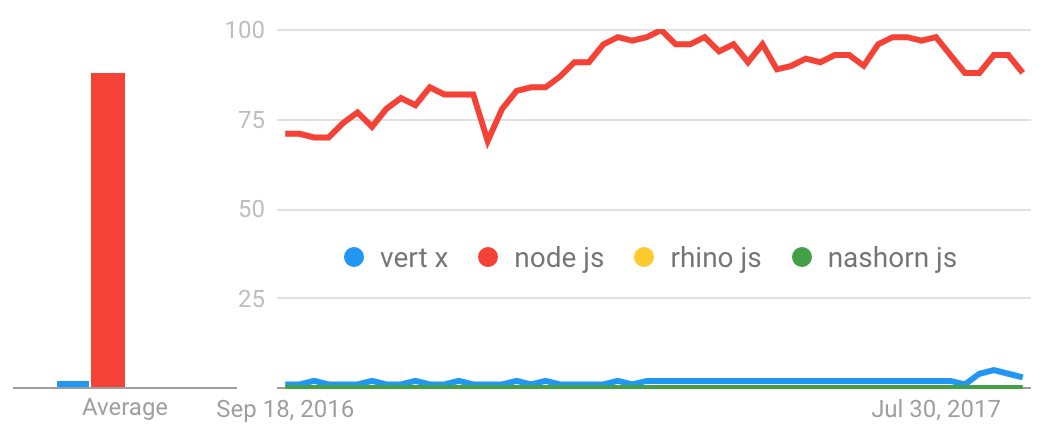
\includegraphics[scale=0.35]{figures/node-vs-other}
\caption{Popularity of Node.js compared to other options to run JavaScript on the server. Measured with Google Trends.}
\end{figure}
While popularity is not always a measure of quality (take for example full stack TypeScript), in this case it seems a little far fetched to consider anything else than Node.js. Writing a full stack TypeScript web-app is already enough risky, in my opinion it wouldn't be wise to make another pioneering move with a choice else than Node.js. Especially since Node.js isn't worse than any of the other options.

Node.js is ``a JavaScript runtime built on Chrome's V8 JavaScript engine'', according to it's own description. This means that it's using the same mechanics to compile JavaScript to machine code as Google Chrome (using V8), but provides a different API. For example, in Chrome you have the \texttt{window} object, which doesn't exist in the Node.js runtime environment. On the other hand, you'll only find the FileSystem API in Node.js, but not Chrome.


\subsection{Performance}
Performance is often an important measure when

\subsection{Production Mode}

\section{Library-Oriented Architecture}

\section{Unit Testing}

\section{Avoiding Callback Hell}

- callbacks
- promises
- Async

e.g. http://callbackhell.com/



\section{Database-Layer}

\subsection{SQL}

\subsection{NoSQL}

\section{Authentication}

\section{Routing}


\chapter{TypeScript in the Frontend}

The way TypeScript is used in the frontend really depends on what you use it with. If you use it with Angular it will be different than when you use it with React. And it's also different when you use it together with VueJS. You see where this is going. With Angular it will be supported 'native' and with React you'll have to learn TSX. Of course, the TypeScript fundamentals will still be the same. But the different frameworks / libraries you'll use will shape your frontend far more than TypeScript does.

\section{TypeScript with Angular}

Having said that, I would like to stress that Angular by far has the best TypeScript community. This is because Angular has TypeScript as a \textbf{default}, where React has JSX as default and VueJS has JavaScript as it's default. Now betting on Angular has proven to be a bad idea in the past with the Google deprecating AngularJS completely\footnote{The framework for versions 1.x is correctly (but confusingly) referred to as AngularJS and newer framework as Angular.}. So where does this leave us with the newer Angular framework? It's still not a safe bet. Nothing ever is in the fast moving frontend world. But it's  a modular and scalable, performant and feature rich framework that's backed by a big company. If you want to build a scalable application in TypeScript, it's one of the best shots you've got.


\section{TypeScript with React}

- TSX

- What's the percentage of ppl using TSX?

...


\section{TypeScript with VueJS}

...

\section{Vanilla TypeScript}


\chapter{A Starter / Seed / Boilerplate for Full Stack TypeScript}

As a bonus to the book, there's a starter-kit / seed / boilerplate available online. The idea behind is the following: \textbf{All web-apps are roughly the same}. Let me elaborate this. Usually, a web-app revolves around one main "object". For example, for Youtube this would be videos, for Twitter tweets, for Instagram images and for Wunderlist it's todos. The whole app consists of users viewing or modifying those objects or lists of those objects. Thus it's possible to build a seed, that covers the basic needs of almost every web-app.

Using the starter has another benefit, than just getting started faster. You're also getting started \textit{better}. We've spent months on perfecting the foundation for your next web-app. We've thought through the architecture, security, performance and monitoring concerns of your application. Now having such an elaborate starter adds a certain complexity to it. It's nothing for complete beginners. But with a fundamental understanding of TypeScript and having read through this book, you're to dive into the starter.

What's a starter, anyways? It's code to get you started. It's maybe best illustrated in light of what it's actually not. It's not a framework and it's not a library. Frameworks and libraries receive regular updates that you are \textit{supposed} to use. As opposed to this, once you've started using the tsmean starter, you won't be relying on updates from us anymore. You can change everything about the starter. You don't have to stay backwards compatible. The idea is really just to provide you a headstart with good architecture and save you the initial weeks of setup, but from then on, you're on your own. Having said this, that doesn't mean that the starter doesn't \textit{make use of libraries}. There are several libraries and frameworks at play in the starter, most notably Angular in the Frontend and ExpressJS in the backend.

\section{Why MEAN?}
...

\section {Getting started with the starter}
Despite the elaborate architecture and feature set of the starter, we tried keeping getting started as simple as possible. You can install everything with a few simple command line promts:

[XXX insert promts here]

\chapter{Deployment}

\subsection{Continuous Integration}

\chapter{Epilogue}

Thanks for coming along the ride. I hope I could introduce you to the new and exciting world of full stack TypeScript.

\begin{thebibliography}{9}

\bibitem{lamport94}
  Baishakhi Ray, Daryl Posnett, Vladimir Filkov, Premkumar Devanbu,
  \textit{A Large Scale Study of Programming Languages
and Code Quality in Github},
  Department of Computer Science, University of California, Davis, CA, 95616, USA

\end{thebibliography}
\end{document}
\begin{document}



\end{document}
\begin{document}



\end{document}
\begin{document}



\end{document}
\begin{document}



\end{document}
\begin{document}



\end{document}
\begin{document}



\end{document}
\begin{document}



\end{document}
\begin{document}



\end{document}
\begin{document}



\end{document}
